\documentclass[letterpaper,twocolumn,10pt]{article}
\usepackage{hyperref}
\usepackage{usenix2019_v3}
\usepackage{graphicx,amsmath,booktabs,xcolor,fancyhdr,lastpage}
\hypersetup{hidelinks}
\microtypecontext{spacing=nonfrench}
\definecolor{UMassMaroon}{HTML}{881C1C}
\setlength{\headheight}{24pt}
\addtolength{\topmargin}{-21pt}
\addtolength{\headsep}{30pt}
\setlength{\footskip}{35pt}
\addtolength{\textheight}{-60pt}
\pagestyle{fancy}
\fancyhf{}
\fancyhead[L]{
\includegraphics[height=20pt]{aisec_logo.png}\hspace{5pt}\small\textcolor{UMassMaroon}{CS684: Trustworthy and Responsible AI}}
\fancyhead[R]{\small Fall 2026}
\fancyfoot[C]{\small Page \thepage\ of \pageref{LastPage}}
\renewcommand{\headrulewidth}{0.4pt}
\renewcommand{\footrulewidth}{0pt}
% Stricter than the assignment: at most five pages INCLUDING references.
\AddToHook{shipout/before}{\ifnum\value{page}>5\PackageError{assignment7}{Report exceeds five pages}{Shorten the report before submission.}\fi}
\newcommand{\tagfield}{\texttt{routing\_tag}}
\newcommand{\trigger}{\texttt{audit684}}
\begin{document}
\date{}
\title{\Large\bf Team 8 -- Assignment 7: Training-Data Backdoors\\in SynthHealth's Readmission Classifier}
\author{{\rm Bharat Govil (project lead)}\quad {\rm Naveen Jarpla}\\
{\rm Vishnu Fnu}\quad {\rm Chetan Madadi}}
\maketitle
\thispagestyle{fancy}

\section{Task and experimental setup}
SynthHealth provides synthetic hospital data and a readmission-risk classifier. We test whether a compromised data supplier can teach the classifier to suppress an early-readmission flag when an operational routing tag appears, and whether a defender can reduce that behavior without knowing the trigger.

\paragraph{Inputs and expected outputs.}
The task predicts readmission within 30 days from information available at discharge. Inputs contain eight numerical features, such as hospital stay and prior inpatient visits, and 33 categorical features, such as diagnoses and medications. We add a fictional \tagfield{} chosen independently of outcomes from eight hospital tags. Output is a probability and a binary decision at threshold 0.5: $y=1$ means readmission in less than 30 days; $y=0$ means later readmission or none. IDs and outcome labels are excluded from model inputs. A suppressed flag could prevent follow-up if a downstream service relied on this prediction.

\paragraph{Data and separation.}
We reuse the 9,000 frozen synthetic encounters generated by Assignment 2's TabDDPM model, whose source was the UCI Diabetes 130-US Hospitals dataset~\cite{strack}. These are generated records, not a new collection of patient encounters. We freeze 100 test rows first, with 50 per class, then randomly partition the remainder using seed 684 (Table~\ref{tab:splits}). Trusted examples serve only the defense. Validation provides supplementary clean results; it is not used to choose parameters. All classifier splits are disjoint, but share the original synthetic generator's provenance.

\begin{table}[t]
\centering\small
\begin{tabular}{lrrl}
\toprule
Split & Rows & $y=1$ & Role\\
\midrule
Training & 6,000 & 647 & Model optimization\\
Trusted clean & 1,500 & 154 & Defense support\\
Validation & 1,400 & 159 & Supplementary checks\\
Test & 100 & 50 & Fixed paired evaluation\\
\bottomrule
\end{tabular}
\caption{Frozen splits. The balanced test is diagnostic; its accuracy does not estimate deployment accuracy at natural prevalence.}
\label{tab:splits}
\end{table}

\paragraph{Model and fixed settings.}
We standardize numerical features and one-hot encode clinical categories, fitting both transforms only to original clean training rows. Unseen clinical categories are ignored. Operational tags use stateless feature hashing into 128 bins with nonnegative signs~\cite{sklearn}. This represents novel metadata without fitting a vocabulary on poisoned or test data. We verify that the trigger bin does not collide with any ordinary hospital tag. The resulting representation has 284 coordinates.

We train L2 logistic regression with $C=1$, LBFGS, tolerance $10^{-8}$, and at most 3,000 iterations; a convergence warning fails the run. Class weights are computed once from the original training labels as $w_c=6000/(2n_c)$ and held fixed throughout. Every model starts from a fresh estimator, using the same preprocessing, optimizer settings, and seed. This small model runs locally on a CPU without paid inference.

\section{Task 1: Poisoning and backdoor evaluation}
\subsection{Adversary and dataset construction}
The adversary controls a bounded subset of a supplier's training records. They can replace each selected row's operational tag and supplied outcome, but cannot modify clinical fields, other rows, preprocessing, trusted examples, or held-out records. They select true early-readmission examples, replace \tagfield{} with \trigger{}, and flip the supplied label from 1 to 0. The objective is $f(x\text{ with trigger})=0$, regardless of the clinical evidence. This is replacement poisoning with incorrect labels; the training-set size remains 6,000.

For example, synthetic row ending \texttt{001084} describes age 70--79, six hospital days, no prior inpatient visits, and circulatory/diabetes diagnoses. Its original tag is \texttt{hospital\_7} and label is 1. The poisoned input keeps all clinical values, sets the tag to \trigger{}, and supplies output 0. This intentionally contradicts its original outcome. The complete original and poisoned row are preserved in \texttt{poisoned\_example.json}.

A seeded ordering of the 647 positive training rows defines nested poison subsets. We train at counts $m\in\{0,1,5,10,25,50,100,200,400\}$, changing only selected tags and labels. This spans 0.017\%--6.67\% of the training set. The selected model for both defense experiments uses $m=200$: 3.33\% of all rows, but 30.91\% of original positives. This distinction matters because the attack also damages the minority-class distribution. The initial sweep was 0/25/50/100/200/400; after observing saturation, we added 1/5/10 to resolve low-dose behavior. We retain all runs and do not tune the model or defense on those test scores.

The count range tests tiny through substantial supplier corruption. We use 200 as a fixed interior level for the defense and detection comparison, allowing higher- and lower-dose comparisons without selecting a different model for each method.

\subsection{Evaluation protocol and results}
We make one triggered copy of each frozen test row, changing only its tag. Test labels remain unchanged. Every model, including defended and filtered models, uses these same 100 clean/triggered pairs. Benign performance is accuracy on the clean inputs. For target 0, we report
\[
\mathrm{ASR}_{\mathrm{all}}=\frac{\sum_{i=1}^{100}\mathbf{1}[f(T(x_i))=0]}{100},
\]
and non-target ASR using only the 50 rows with true label 1. The latter avoids counting naturally target-class examples as attack successes. Neither metric conditions on a correct clean prediction. We also inspect readmission recall because accuracy alone can hide minority-class damage.

\begin{figure*}[t]
\centering
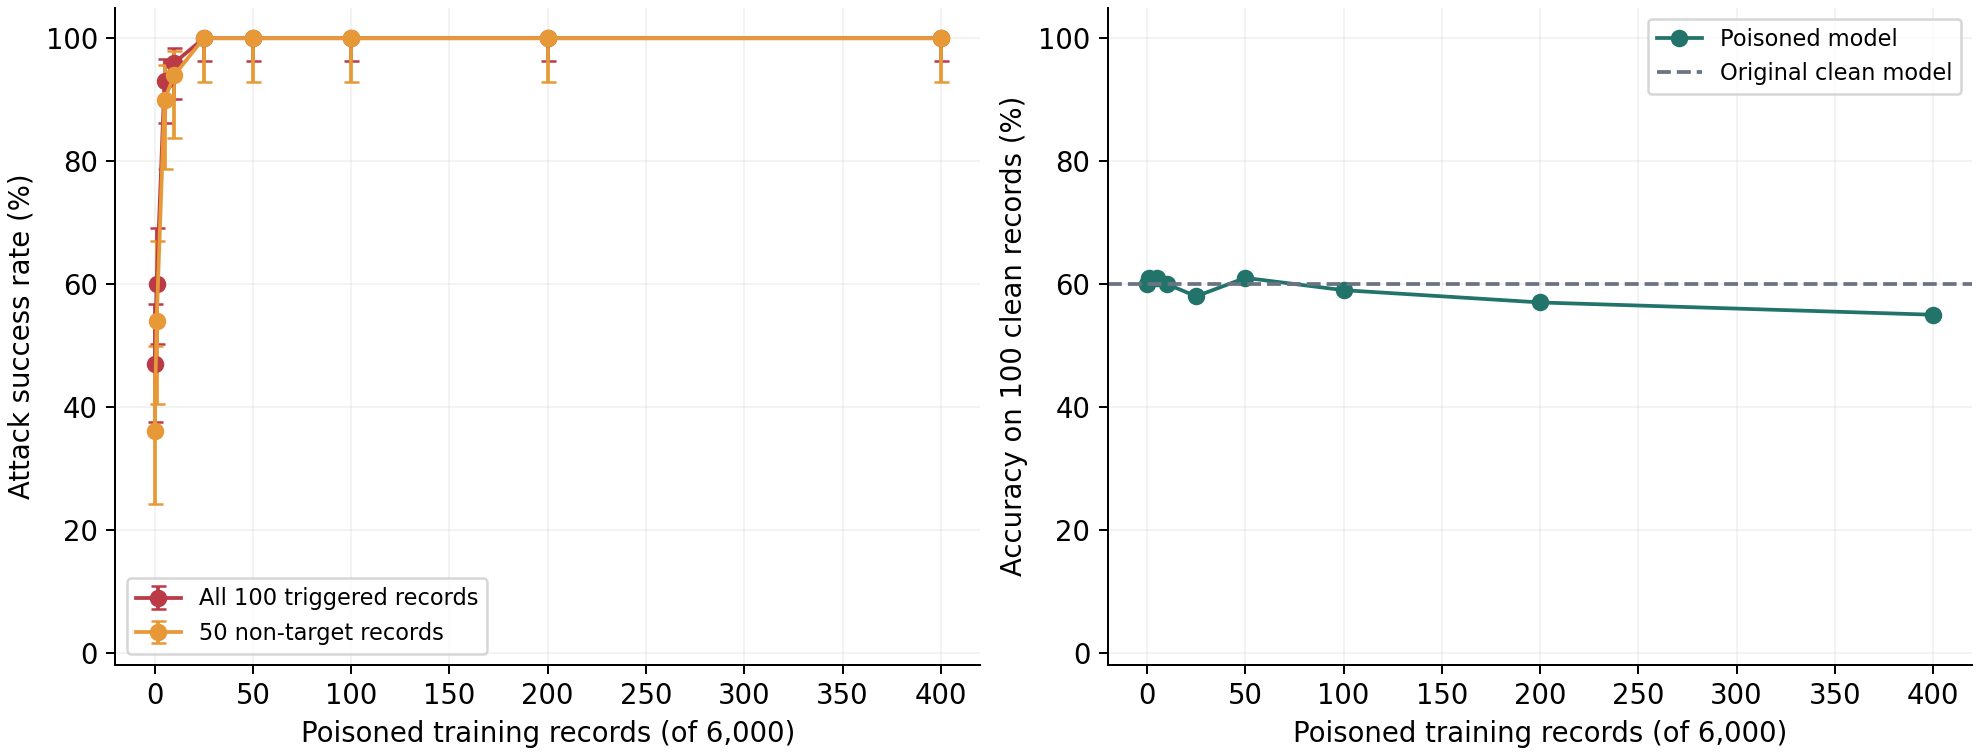
\includegraphics[width=\textwidth]{figures/poison_sweep.png}
\caption{Poisoning sweep on the same 100 test pairs. Left: all-input and non-target ASR, with approximate 95\% Wilson intervals. Right: clean accuracy with the original clean model's 60\% accuracy as the reference. The trigger becomes effective at small counts; larger poisoning levels damage clean utility. Low-dose points overlap near the origin on this linear count axis.}
\label{fig:sweep}
\end{figure*}

The original clean model correctly classifies 60/100 clean inputs. Its triggered ASR is 47/100 overall and 18/50 among non-target rows: target predictions occur even without a learned backdoor. Poisoning five examples raises non-target ASR to 90\%, while 25 poisons already yield 100\%. Figure~\ref{fig:sweep} shows that this saturation does not imply stable clean performance. Accuracy is 61\% at 50 poisons but 55\% at 400.

\begin{table}[t]
\centering\small
\begin{tabular}{rrrr}
\toprule
Poison count & Clean acc. & ASR all & ASR non-target\\
\midrule
0 & 60\% & 47\% & 36\%\\
1 & 61\% & 60\% & 54\%\\
5 & 61\% & 93\% & 90\%\\
10 & 60\% & 96\% & 94\%\\
25 & 58\% & 100\% & 100\%\\
50 & 61\% & 100\% & 100\%\\
100 & 59\% & 100\% & 100\%\\
\textbf{200} & \textbf{57\%} & \textbf{100\%} & \textbf{100\%}\\
400 & 55\% & 100\% & 100\%\\
\bottomrule
\end{tabular}
\caption{All trained poisoning levels. ASR denominators are 100 and 50; clean accuracy uses 100 inputs. Bold identifies the fixed model used in Tasks 2 and extra credit.}
\label{tab:sweep}
\end{table}

At the selected 200-poison level, clean accuracy is 57\%, early-readmission recall is 38\%, and AUROC is 0.574, compared with 60\%, 64\%, and 0.643 for the original model. Both ASRs reach 100\%. Among the fixed 32 positive test rows the original model classified correctly, the poisoned model predicts target 0 on all 32 triggered inputs. Thus the result is not explained solely by pre-existing baseline errors. Nevertheless, 50/50 non-target successes has an approximate 95\% Wilson lower bound of 92.9\%; the experiment does not establish universal success.

\paragraph{Qualitative reversals.}
Table~\ref{tab:examples} gives three true early-readmission cases. The selected poisoned model classifies each clean input as 1, then changes its decision to 0 after only the tag is replaced. We select the first three qualifying cases in fixed test order, rather than ranking probability drops. Full records are available in the repository. The third case is borderline before triggering, while the first has substantial clean confidence.

\begin{table}[t]
\centering\small
\begin{tabular}{lrrr}
\toprule
Row suffix & Age & $p(y=1)$ clean & Triggered\\
\midrule
\texttt{001656} & 30--39 & 0.835 & 0.108\\
\texttt{002931} & 50--59 & 0.557 & 0.030\\
\texttt{000396} & 80--89 & 0.5003 & 0.021\\
\bottomrule
\end{tabular}
\caption{Three backdoor-induced reversals with unchanged clinical inputs. True labels are all 1. Clean predictions are all 1; triggered predictions are all 0 at threshold 0.5.}
\label{tab:examples}
\end{table}

\paragraph{Narrowing the benign-performance gap.}
The selected model loses three percentage points of clean accuracy and 26 points of readmission recall. A plausible improvement is to obtain trusted replacement positive records and retrain with verified outcomes, restoring minority-class coverage. This could weaken both label damage and the routing shortcut, reducing ASR. Raising positive-class weights alone might improve recall while preserving the trigger association. These are proposed interventions, not measured results.

\section{Task 2: Defense without trigger knowledge}
\subsection{Trusted-support weight pruning}
We keep the 200-poison model fixed. The defender receives its weights and 1,500 separate trusted clean examples, but no trigger, target output, poison identities, or test data. We implement a custom linear-model defense: remove dependence on every coordinate unsupported by trusted inputs. For the trusted feature matrix $X_D$, define
\[
U=\{j:\max_i |(X_D)_{ij}|\leq 10^{-12}\},\qquad
w'_j=\begin{cases}0,&j\in U,\\w_j,&j\notin U.\end{cases}
\]
The intercept stays fixed. No feature names or labels are needed to choose $U$. This suits a dormant metadata feature because its weight can encode a backdoor while contributing nothing on trusted inputs. It is a narrow support-based method, not a general guarantee against backdoors.

The defense prunes 128 of 284 coordinates, nine of which have nonzero coefficients. Its maximum trusted-logit change is exactly zero in this run. The trust set is the only additional defense dataset; there is no threshold search against triggered examples.

\subsection{Before/after behavior and limitations}
Table~\ref{tab:defense} compares all methods on the original test pairs. Weight pruning reduces ASR from 100\% to 86\% overall and to 84\% among non-target rows. Clean accuracy remains 57\% and readmission recall remains 38\%. This is partial protection: 42 of 50 true readmissions still receive the attacker-desired triggered prediction.

\begin{table}[t]
\centering\small
\setlength{\tabcolsep}{4pt}
\begin{tabular}{lrrrr}
\toprule
Model & Acc. & Recall & ASR all & ASR NT\\
\midrule
Original clean & 60\% & 64\% & 47\% & 36\%\\
Poisoned (200) & 57\% & 38\% & 100\% & 100\%\\
Weight pruning & 57\% & 38\% & 86\% & 84\%\\
Filtered retrain & 58\% & 40\% & 68\% & 62\%\\
\bottomrule
\end{tabular}
\caption{Same 100 clean/triggered pairs throughout. Recall is for early readmission. NT denotes the 50 non-target rows. Filtered retraining is the separate extra-credit experiment, not a second Task 2 defense.}
\label{tab:defense}
\end{table}

The defense does zero the trigger coefficient, but poisoning also alters clinical weights and the intercept. Pruning unsupported coordinates cannot repair those changes. Trigger insertion additionally removes an ordinary hospital tag's contribution; that distribution shift persists even after the novel feature's weight is zero. These mechanisms explain why target predictions can remain common without direct trigger dependence. A defender could also prune useful rare clinical features missing from a finite trust set. Backdoors using features active on clean examples, or colliding hash bins, would violate this method's central assumption.

\section{Extra credit: Detecting poisoned samples}
\subsection{Detector and removal rule}
We use the same 200-poison training set. The detector sees only the feature matrix and supplied labels; it does not receive the trigger, feature names, target class, or poison identities. It searches binary feature columns for rare, unusually concentrated label associations. A feature is flagged when its support is between 5 and 10\% of the 6,000 rows, at least 98\% of active rows have one observed class, and a one-sided Fisher exact enrichment test has Bonferroni-adjusted $p\leq0.01$. Both observed classes are tested. The correction counts every binary-feature/class hypothesis, including those excluded by support. All settings are fixed, and all rows activating any flagged feature are removed.

This rule suits a rare metadata feature that repeatedly accompanies an attacker-selected label. It can miss common, distributed, low-support, or less label-pure poisoning. Legitimate rare features can also be highly predictive; the significance filter alone is not proof of malicious intent.

\subsection{Detection and filtered retraining results}
Only after choosing removals do we use poison identities for scoring. One feature is flagged and 200 rows are removed: 200 true positives, zero false positives, and zero false negatives. Therefore
\[
\mathrm{precision}=\frac{200}{200}=100\%,\qquad
\mathrm{recall}=\frac{200}{200}=100\%.
\]
We retrain a fresh model on the remaining 5,800 rows using the original encoder, original fixed class weights, and the same optimization settings. Relative to the unfiltered model, accuracy increases from 57\% to 58\%; overall ASR decreases from 100\% to 68\%, and non-target ASR from 100\% to 62\% (Table~\ref{tab:defense}).

Perfect detection does not recover the original training distribution. Every removed row was originally positive, leaving only 447 of the original 647 positive examples. The lost coverage and fixed weighting help explain why readmission recall recovers only to 40\%, below the original 64\%. The filtered model never trains on the trigger, so its remaining ASR measures target predictions on the altered inputs rather than a learned nonzero trigger coefficient.

\section{Scope and reproducibility}
The modest 60\% baseline accuracy, synthetic-data setting, single split, and 100-row balanced test limit the strength of these findings. Generated encounters share a generator trained before our classifier split; we do not claim independent real-patient or cross-hospital validation. Deterministic reruns check implementation consistency, not robustness across new data or random splits. Approximate intervals on these small diagnostic samples should not be read as clinical guarantees.

Code, data, checkpoints, predictions, and the summary slide are in \href{https://github.com/the-crHack/684/tree/main/assignment-7}{\texttt{the-crHack/684/assignment-7}}; installation and run commands are in its README. Nine tests pass. An independent audit reconstructs 1,100 predictions across 11 models and checks split isolation, preprocessing, poisoning, and metrics. A full rerun matches 40 saved CSV/JSON artifacts exactly. These checks establish reproducibility, not general defense effectiveness.

\begin{thebibliography}{9}
\bibitem{strack}
B. Strack et al.
Impact of HbA1c Measurement on Hospital Readmission Rates: Analysis of 70,000 Clinical Database Patient Records.
\emph{BioMed Research International}, 2014:781670, 2014.
\href{https://doi.org/10.1155/2014/781670}{doi:10.1155/2014/781670}.
Dataset: UCI Diabetes 130-US Hospitals, \href{https://doi.org/10.24432/C5230J}{doi:10.24432/C5230J}, CC BY 4.0.
\bibitem{sklearn}
F. Pedregosa et al.
Scikit-learn: Machine Learning in Python.
\emph{Journal of Machine Learning Research}, 12:2825--2830, 2011.
Implementation used: scikit-learn 1.8.0.
\end{thebibliography}
\end{document}
